% Chapter Template

\chapter{Conclusion} % Main chapter title

\label{Chapter7} % Change X to a consecutive number; for referencing this
% chapter elsewhere, use \ref{ChapterX}

\lhead{Chapter 7. \emph{Conclusion}} % Change X to a consecutive

There are several model transformation environments available that provides
model to model transformations. These environments are designed accordingly
to different approaches to model transformations. In this thesis we have
explored three different model transformation environments that could expand the
DPF Workbench with model to model transformation. We implemented a version of
the DPF Transformation Editor that integrates the Henshin transformation language
to provide an exogenous model transformation environment for DPF.
This is something to consider though, because even though the DPF Transformation
Editor provides support for exogenous model transformations the language syntax
of DPF remains the same before and after the execution of a set of
transformation rules. This means that without the ontological meta-models we
could not extend a tool with support for exogenous model transformations.
However, since we can include modeling formalisms at different layers of
abstraction with the help of application conditions, Henshin proved to be a
viable transformation language that facilitates a model to model transformation
environment for the DPF Workbench. In this thesis we have explained that
Henshin can be extended with application conditions to perform model
transformations on models described through arbitrary layers of abstractions.

\begin{itemize}
  \item Henshin requires application conditions to specify the abstract
  syntax from a DPF specification one abstraction layer higher.
   \item Henshin requires a traceable link between each source and target
   modeling elements. This traceable link is utilized in three different aspects when
  integrating Henshin with the DPF Transformation Editor. 
	\begin{enumerate} 
	  	\item Specifies that the engine only translates a matching pattern once.
        \item Defines a correspondence between source and target modeling
        elements. 
        \item Reusable in other rules if the source and target element are used
        to define the LHS and RHS graph.
     \end{enumerate}
     
\end{itemize}

For an exogenous model transformation Henshin requires a traceable
link between source and target modeling elements not only to specify the
correspondence between two modeling objects, but also to reuse the source and
target node of this traceable links in other rules. These modeling objects
represents either a node or an arrow in a DPF specification. For a
transformation rule when a traceable link is first established it is actually
transformed like any other graph structure initialized by the RHS graph. Now we
can use this traceable link between modeling elements in other transformation
rules. Note that to use a traceable link in other rules can result in potential
dependency issues. This is because for the editor we designed
the application control mechanism to apply transformation rules in a sequential
order. If the application control utilizes a non-deterministic mechanism to
apply rules then the target model would in worst case not produce any
result, since one rule requires a traceable link that should be initialized in
another rule. However, to apply a set of transformation rules
non-deterministically is convenient if the source model contains a dense graph.

The integration of Henshin with DPF allows for the possibility to translate a
DPF specification to a DPF specification that conforms to another modeling
formalism. The solution still requires more testing on different exogenous model
transformation scenarios, but the editor should be able to create a set of
transformation rules in Henshin transformation language based on a source and
target modeling formalism.

\section{Future Work}

There is still some work that is required to be done before the DPF
Transformation Editor becomes a mature system that can provides model to model
transformations.

\subsection{Endogenous Model Transformations}

In this thesis we presented an integration of Henshin that supports exogenous
model transformations over different layers of abstraction, but the DPF
Transformtaion Editor should be extended with endogenous model transformations.
This can also be achieved by using Henshin, but an endogenous model
transformation solution is done differently in Henshin compared to an exogenous
model transformation. For Henshin we can utilize the double pushout approach to
first locate a match, then delete modeling elements that are uniquely part of
the LHS. The next pushout consist of inserting modeling elements that are
uniquely part of the RHS. While these two operations are performed, modeling
elements that is part of both the LHS and the RHS are preserved. This meant that
we do not need traceable links to provide endogenous model transformation on DPF
specifications in Henshin.

\subsection{Constraint Aware Model Transformations}

The DPF Transformation Editor does at this moment not provide model to model
transformation that is constraint aware for the source and target modeling
formalism. This means that we do not consider the constraints that is
defined in the abstract syntax of the source and target meta-model.
Figure~\ref{fig:simple_modeling_formalism_constraints} explains how we can do
this.

\begin{figure}[H]
	\centering
	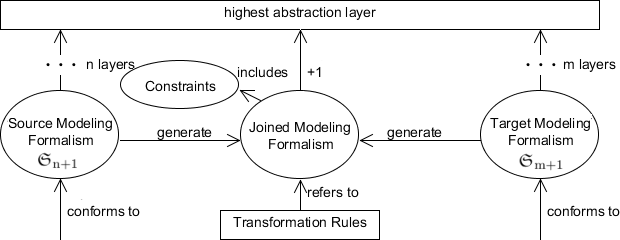
\includegraphics[scale=0.7]{./Figures/simple_modeling_formalism_constraints.png}
	\caption[Simplified joined specification]
	{A simplified joined modeling formalism with constraints that transformation
	rules refers to.}
	\label{fig:simple_modeling_formalism_constraints}
\end{figure}

We could extend the joined modeling formalism with constraints. This means that
we have to create the constraints for both the source modeling formalism and the
target modeling formalism in the joined modeling formalism. This means that we
can make transformation rules in the DPF Transformation Editor that also
includes the possibility to define the RHS with constraints based on constraints
from the LHS. This convenient if we want to transform one modeling formalism
into another modeling formalism.

\subsection{Verification of target modeling formalism predicates}

When the target model is finished with the transformation the corresponding
predicates from the target modeling formalism requires verification. This can be
achieved by searching through every single node and arrow in the target
specification and make sure that the predicates are fulfilled with the target
modeling formalism one abstraction layer higher. 





